% 04a3_attach_offset.tex -- draft 23 Oct 2026. Pending results are \placeholder{}.
\subsection{How far off its plate a newcomer can catch}
\label{sec:res_attach_offset}

A magnet catches wherever its tip is when it fires, which need not be the centre of its plate. The planner of
Section~\ref{sec:attach} therefore folds the newcomer in at the \emph{measured} catch point, the tip's position in
the ring's frame at the catch. We test this choice against folding in at the slot assumed, the plate's nominal
point, in the twin: three carriers hover the ring on 1\,m cables, the newcomer's catch point is moved off its plate
by a set distance $d$, either along the rim toward the neighbouring carrier or radially inward, and the fleet then
flies a figure-eight. Each cell flies twice. A run completes if the newcomer is caught and folded in, the ring's tilt
peak in the fold-in stays under 5$^\circ$, and the fleet finishes its path. Up to about 2.5\,cm the offset is a
real catch error, since a real magnet catches only on its 60\,mm plate; beyond that the sweep measures the fold-in's
tolerance to error in the attach-point model, not how far off a real magnet can catch.

Radially inward the measured catch point holds to the largest offset flown, 16\,cm, with a fold-in tilt peak of at
most 2.63$^\circ$ (Fig.~\ref{fig:attach_offset}, Table~\ref{tab:attach_offset}). Assuming the slot passes the
5$^\circ$ bar from 8\,cm: the planner's balance ignores the moment of the offset, so the ring hangs off its
reference and the newcomer nears its throttle limit, and the tilt grows with the offset to 15--17$^\circ$ at
16\,cm. Here the mechanism is shown: the slot arm's tilt grows with the model error, the measured arm's does not.
Whether the measured arm still holds at 20\,cm is \placeholder{20\,cm radial extension, both arms, owed}.

Along the rim the order reverses past 8\,cm. The measured catch point completes to 6\,cm
(\placeholder{8\,cm if its owed re-fly completes}) and fails the fold-in bar at 11.6\,cm, the next plate's centre,
with tilt peaks of 5.1--8.9$^\circ$ from there to 16\,cm. The slot arm folds in more gently along the rim, peaking at
3.5--4.7$^\circ$ over the same offsets; its own limit, 2\,cm (\placeholder{4\,cm if its owed re-fly completes}), is
set by the twin's weld trigger, which once failed to fire at 6\,cm whatever the arm. Along the rim the mechanism is
therefore not shown. Separation from the neighbouring carrier is reported apart from these limits: folding in at the
measured point moves the newcomer toward that carrier, to 0.22--0.23\,m at 16\,cm, inside the 0.30\,m line, while
the slot arm keeps at least 0.54\,m and every radial run at least 0.64\,m.

\begin{figure}[t]
\centering
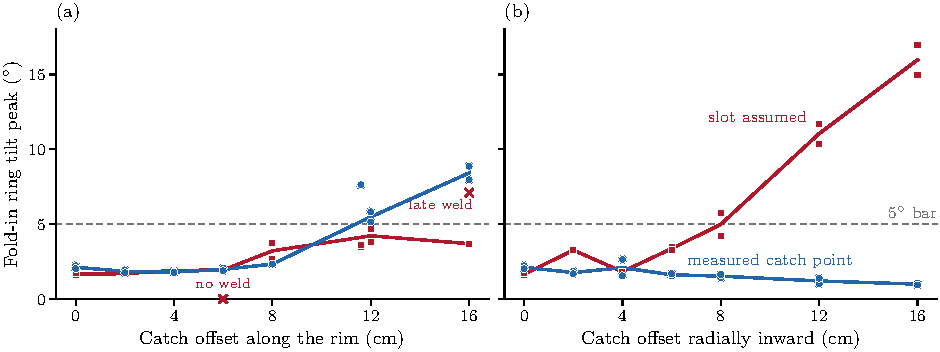
\includegraphics[width=\columnwidth]{figures/fig_u_catch_offset.pdf}
\caption{The ring's tilt peak in the fold-in against the catch offset, folding in at the measured catch point and at
the slot assumed, (a) along the rim and (b) radially inward. One marker per run, the line through the cell means;
crosses mark the slot arm's two weld-trigger failures. The bar is 5$^\circ$. Past about 2.5\,cm the
offset is model error rather than a real catch.}
\label{fig:attach_offset}
\end{figure}

\begin{table}[t]
\centering
\footnotesize
\setlength{\tabcolsep}{4pt}
\caption{Largest catch offset completed within the 5$^\circ$ fold-in bar (two runs a cell, twin, 1\,m cables).}
\label{tab:attach_offset}
\begin{tabular}{lcc}
\toprule
Fold-in point & Radially inward & Along the rim \\
\midrule
Measured catch point & 16\,cm \placeholder{20?} & 6\,cm \placeholder{8?} \\
Slot assumed         & 6\,cm                    & 2\,cm \placeholder{4?} \\
\bottomrule
\end{tabular}
\end{table}
